
To verify whether the differences between MMR and Exp-$1$-call@$k$
matter empirically, we compare the two algorithms across a number of
metrics on three diversity testbeds: the TREC 6-8 Interactive
Track\footnotemark[1] (17 queries) and 2009 and 2010 ClueWeb Diversity
tasks of the TREC Web Track\footnotemark[2] (50 queries each).  On
these testbeds, we evaluate \emph{mean subtopic
recall@$k$}~\cite{zhai03Beyond} (fraction of total annotated
aspects/subtopics covered by a result set at rank $k$, averaged over
queries), which is an appropriate loss function for the
\emph{set-level} metric~\eqref{eq:setRelevance}~\cite{chen06Less}.  We
also evaluate a variety of more recent \emph{rank-based} diversity evaluation
metrics such as intent-aware expected reciprocal rank
(ERR-IA@$k$)~\cite{err-ia}, $\alpha$-nDCG@$k$~\cite{clarke08Novelty},
and intent-aware mean average precision
(MAP-IA)~\cite{agrawal09diversifying}.

We use MMR with $\lambda = 0.5$ to match the equal weighting of
similarity and diversity in Exp-$1$-call@$k$.  An
LDA~\cite{blei03Latent} topic model is trained on the top-100 OKAPI
BM25~\cite{bm25} results for each query (on its respective collection)
and these subtopic distributions are used for the similarity and
diversity kernels in both algorithms: for MMR we choose $\Sim_1$ and
$\Sim_2$ kernels as in~\eqref{eq:sim_term} --- effectively LDA
variants of latent semantic indexing (LSI)~\cite{deerwester90LSA}
kernels; for Exp-$1$-call@$k$, we use the similarity and diversity
kernels respectively defined in~\eqref{eq:sim_term}
and~\eqref{eq:div_term}.  Both MMR and Exp-$1$-call@$k$ are used to
rank the top-20 documents from the top-100 OKAPI BM25 results.

Results in Table~\ref{table:different_metrics} and
Figure~\ref{fig:mmr_vs_1call} show the performances of MMR and
Exp-$1$-call@$k$ on the three diversity testbeds across various
diversity measures; although there are minor performance differences,
we note that these differences are not statistically significant
w.r.t.\ 95\% confidence intervals.  Nonetheless, the results appear to
indicate that the structural similarities in the use of MMR and the
optimization of Exp-$1$-call@$k$ outweigh the differences in this
evaluation.

%%%%%%%%%%%%%%%%%%%%%%%%%%%%%%%%%%%%%%%%%%%%%%%%%%%%%%%%%%%%%%%%%%
{\footnotesize
\begin{table}
\tbl{MMR vs Exp-$1$-call@$k$ on various ranking measures of diversity.}{
\begin{tabular}{ll c c c c c c c c }
%\begin{tabular}{|ll|c|c|c|c|c|c|c|c|}
\hline
 % after \\: \hline or \cline{col1-col2} \cline{col3-col4} ...
Testbed & Algorithm & ERR-IA@5 & ERR-IA@10 & ERR-IA@20 & $\alpha$-nDCG@5 & $\alpha$-nDCG@10 & $\alpha$-nDCG@20 & MAP-IA \\ % NRBP & 
\hline \hline
TREC6-8&MMR ($\lambda=.5$) & 0.0433 & 0.0548 & 0.0607 & 0.2310 & 0.2590 & 0.2728 & 0.0361\\ %\hline % & 0.0413 
        & Exp-1-call@$k$ & 0.0456 & 0.0561 & 0.0621 & 0.2332 & 0.2602 & 0.2750 & 0.0365\\ \hline %\hline % & 0.0432
ClueWeb 2009& MMR ($\lambda=.5$) & 0.0984 & 0.1085 & 0.1174 & 0.1500 & 0.1696 & 0.2045 & 0.0095\\ %\hline % & 0.0895 
             & Exp-1-call@$k$ & 0.0972 & 0.1084 & 0.1158 & 0.1435 & 0.1698 & 0.1997 & 0.0123\\ \hline %\hline % & 0.0901 
ClueWeb 2010& MMR ($\lambda=.5$) & 0.1198 & 0.1422 & 0.1503 & 0.1516 & 0.2066 & 0.2339 & 0.0085\\ %\hline % & 0.1125 
             & Exp-1-call@$k$ & 0.1211 & 0.1408 & 0.1550 & 0.1527 & 0.1984 & 0.2476 & 0.0093 \\ \hline % & 0.1147
\end{tabular}}
\label{table:different_metrics}
\end{table}}
%%%%%%%%%%%%%%%%%%%%%%%%%%%%%%%%%%%%%%%%%%%%%%%%%%%%%%%%%%%%%%%%%%

%%%%%%%%%%%%%%%%%%%%%%%%%%%%%%%%%%%%%%%%%%%%%%%%%%%%%%%%%%%%%%%%%%
\begin{figure}[t!]
\centerline{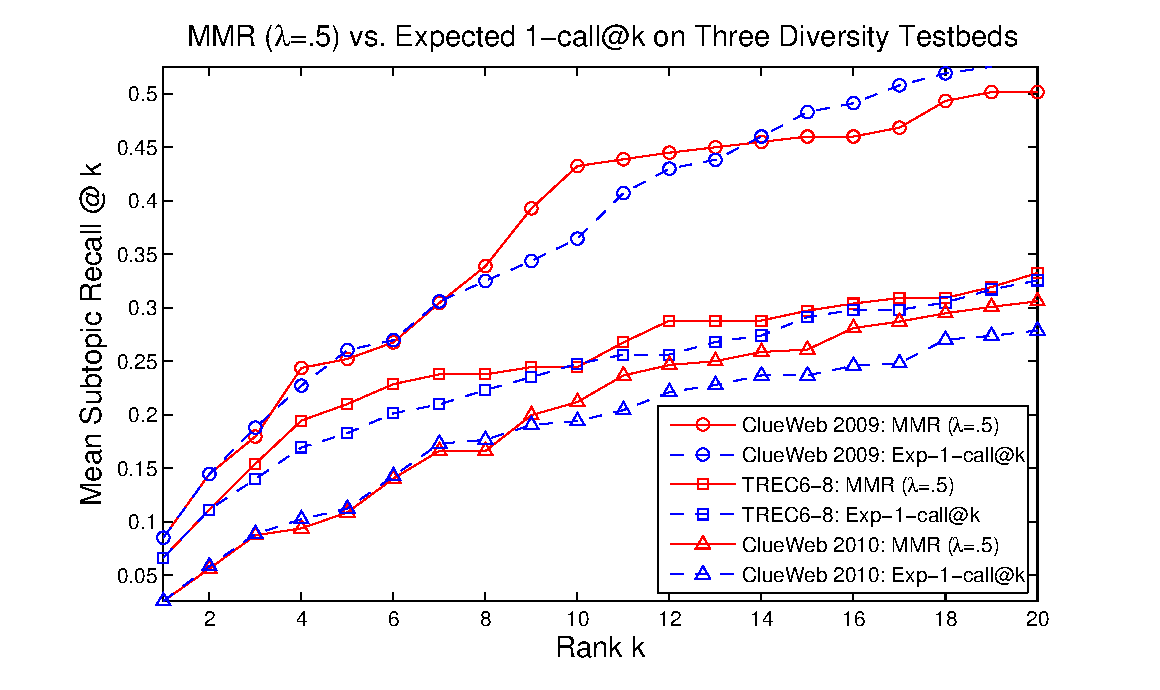
\includegraphics[scale = .65]{mmr_vs_1call}}
\vspace{-3mm}
\caption{MMR vs Exp-$1$-call@$k$ on subtopic recall.}
\label{fig:mmr_vs_1call}
\vspace{-3mm}
\end{figure}
%%%%%%%%%%%%%%%%%%%%%%%%%%%%%%%%%%%%%%%%%%%%%%%%%%%%%%%%%%%%%%%%%%
